
\chapter{Marco conceptual}
\label{mconceptual}

\section{Terminología}
En esta sección, se clarifican aquellos términos que se consideran propios del ámbito estudiado y que permiten entender las ideas que se presentan en los siguiente capítulos.

\begin{itemize}
	
	\item Aitué \cite{ref5}: El significado de esta palabra en español es: "La tierra que uno ama". Esta palabra es nativa del Quechua. 
	\item NCFAS \cite{VALENCIA2010}: Esta sigla que proviene de "North Carolina Family Assessment Scale". La cual en español signigica: "Escala de Evaluación Familiar de Carolina del Norte". Es una herramienta que apoya a los profesionales para poder realizar una apreciación de la situación familiar. 
	\item TIC \cite{almenara2007impacto}: Esta sigla significa Tecnologías de Información y Comunicación. \textit{En líneas generales podríamos decir que las nuevas tecnologías de la información y comunicación son las que giran en torno a tres medios básicos: la informática, la microelectrónica y las telecomunicaciones; pero giran, no sólo de forma aislada, sino lo que es más significativo de manera interactiva y interconexionadas, lo que permite conseguir nuevas realidades comunicativas.}
	\item Minería de Datos \cite{lopez2007mineria}: La minería de datos puede definirse inicialmente, como un proceso de descubrimiento de nuevas y significativas relaciones, patrones y tendencias al examinar grandes cantidades de datos. 
	\item Estadística Descriptiva \cite{alicia2010correlacion}: La estadística descriptiva es un conjunto de procedimientos que tienen por objeto presentar datos por medio de tablas, gráficos y/o medidas de resumen. De acuerdo a lo anterior, la Estadística Descriptiva es la primera etapa a desarrollar en un análisis de información.
	
	\item Competencias Parentales \cite{rodrigo2008preservacion}: pueden ser definidas como el conjunto de capacidades que permiten a los padres afrontar de modo flexible y adaptativo su rol, de acuerdo con las necesidades evolutivas y educativas de sus hijos y bajo los estándares considerados como aceptables por la sociedad, aprovechando todas las oportunidades y apoyos que les brindan los sistemas de influencia de la familia para desplegar dichas capacidades.
	
\end{itemize}

\newpage
\section{Definición del área del problema} \label{contexto}
\vspace{2mm}
\normalsize

En esta sección se contextualiza el área del problema, indicando por que nacen corporaciones que buscan defender los derechos fundamentales de los niños, niñas y adolescentes y además explicar una de las herramientas utilizada por los profesionales que trabajan en estas corporaciones.


\subsection{Vulneraciones de los Derechos de Niños, Niñas y Adolescentes}
\label{vulneraciones}
\vspace{2mm}
\normalsize

Algunos NNA están expuestos a vulneraciones de sus derechos, y estas vulneraciones muchas veces provienen del contexto familiar, los cuales pueden resultar ser patrones generacionales de negligencias, maltratos, resolución violenta de los conflictos, dinámicas relacionales caóticas, todo lo cual provoca en el NNA trastornos en su desarrollo y la manifestación de conductas violentas, tal como señala el Neuro Psiquiatra Jorge Barudy:\\
\textit{Existen diferentes investigaciones realizadas en el campo de la neurología, la etología humana y las neurociencias entregan la información necesaria, para que no quede ninguna duda que la maduración del cerebro y del sistema nervioso de los infantes, depende del cariño, la estimulación y los cuidados que reciben del mundo adulto en especial de sus madres y padres. Cuando esto no ocurre existe un enorme riesgo de daños de las diferentes funciones mentales necesarias para asegurar el aprendizaje, una adaptación sana al entorno y la participación en relaciones interpersonales afectivas basadas en el respeto y la reciprocidad en la producción de cuidados. Por esta razón, insistiremos que los buenos tratos, sobre todo, antes de los tres años de edad, son fundamentales para promover una infancia y una adolescencia sana , así como una adultez, constructiva y altruista. A diferencia de las dinámicas socio familiares que producen malos tratos, las dinámicas de buen trato no producen sufrimiento, ni vulneración de derechos y daños a los niños ni a los jóvenes, sino al contrario, bienestar, salud, así como recursos resilientes.} \cite{REF1}\\

\subsection{PIB}
\vspace{2mm}
\normalsize

Principalmente por estos motivos mencionados en la sección \ref{vulneraciones} se creó el  programa PIB (Programa de Intervención Breve) el cual es un concurso de licitación publica correspondiente a la línea de Programas de Protección en General, nace en el año 2007 con el propósito de “Resolver las vulneraciones de derecho asociadas a situaciones de mediana complejidad que afectan a NNA de un territorio determinado, previniendo su cronificación”. Se refería a mediana complejidad a: “La presencia de situaciones y/o conductas que se constituyen en evidentes señales de alerta de cronificación de vulneraciones de derechos ya presentes, que provocan daño y/o amenazan los derechos de NNA, y que se manifiestan en diversos ámbitos de la vida de éstos, ya sea a nivel personal, familiar y/o socio-comunitario” \cite{REF2} . Estas situaciones hasta ese momento, no estaban siendo abordadas. Sumado a lo anterior, se requería un programa al cual pudieran derivar las Oficinas de Protección de Derechos, OPD y, así, descongestionar su eje de protección de derechos vulnerados.

\subsection{PPF}
\vspace{2mm}
\normalsize

Hoy en día, la red de colaboradores del SENAME, licita bajo la modalidad PPF (Programa de Prevención Focalizada), que es la evolución de la linea preventiva del SENAME y pretende dar continuidad a los avances y aprendizajes de los PIB, así como también, incorporar los ajustes necesarios para mejorar la calidad de la intervención con los NNA y sus familias.

\subsubsection{PPF Aitué}
\label{ppf}
\vspace{2mm}
\normalsize
En el territorio Chileno, en las diferentes ciudades y comunas existen una gran cantidad de Programas de Prevención Focalizada, destinados a acoger a familias de sectores específicos del país.Sin embargo el sistema propuesto se desarrollará en el PPF ubicado en la Región de Valparaíso, específicamente en Viña del Mar en la población Forestal Alto. Ahí se encuentra ubicado el PPF Aitué. Este PPF tiene como finalidad de entregar a los adultos responsables de los NNA capacidad de apegarse a sus hijos/as, modelos de crianza bien tratantes, la capacidad de participar en redes, entrega de recursos destinados a influenciar positivamente las competencias parentales, ya sea promoviendo su adquisición, facilitando sus mejores o rehabilitándolas cuando sea necesario. Al mismo tiempo facilitar a los NNA modelos más sanos para la crianza de sus futuros hijos/as.\\

Esta institución, atiende a NNA entre 0 y 18 años  y su adulto a cargo, habitantes del sector de Forestal Alto y Chorrillos, sin discriminación étnica, religiosa o cultural que presenten vulneraciones de derechos relacionadas con su contexto familiar, de carácter moderado tales como:

\begin{itemize}
	\item Testigos de violencia intrafamiliar no constitutiva de delitos
	\item Maltrato psicológico leve a moderado
	\item Maltrato físico leve a moderado sin denuncias actuales en fiscalía o carabineros
	\item Negligencia moderada, no crónica
	\item Trabajo infantil no correspondiente a peores formas, tales como trabajo en Ferias Libres, comercio callejero u otras de iniciativa propia para satisfacer necesidades específicas y/o como apoyo al sustento económico cuando es precario
	\item Otras vulneraciones de derecho que afecten a NNA y relacionadas con el entorno familiar, no constitutivas de delitos.
	
\end{itemize} 

Esta institución además incluye en la atención a NNA con necesidades especiales tales como Síndrome de Déficit Atencional (SDA) y/o Déficit Intelectual Leve (DIL), los que presentan vulneraciones asociadas a sus necesidades por la falta de herramientas de sus adultos cuidadores respecto al manejo conductual o apoyo en el aprendizaje en general.
Unas de las principales características de los sujetos de atención de esta institución, en el ámbito individual son:
Conductas agresivas, de ineficacia en el auto-control, dificultades para respetar normas y límites, impulsividad y baja tolerancia a la frustración; recursos personales insuficientes para el diálogo y resolución de problemas; bajo rendimiento con sensación de inutilidad y desmotivación en el ámbito escolar; escaso desarrollo de la creatividad; a nivel emocional se observa bajos niveles de autoestima; dificultades para reconocer y expresar sentimientos y emociones, escasas habilidades sociales.\\

En el ámbito familiar dinámicas relacionales basadas en la violencia física y verbal, con descalificaciones u omisiones; dificultades en el establecimiento de límites; utilización de la violencia como principales formas de disciplina; bajos niveles de sensibilidad parental, es decir falta de una adecuada lectura, interpretación o respuestas a necesidades del NNA según características y etapa evolutiva y patrones transgeneracionales de negligencia; significados predominantemente negativos y traumáticos asociados a la crianza; consumo de alcohol y/o drogas entre los adultos significativos; debilitamiento de otras figuras significativas protectoras; familias con jefatura centrada en la mujer con conflictos entre las funciones normativas y nutricias, sumado a un debilitamiento de la autoridad masculina y ausencia de modelos masculinos referentes de tipo positivo y participantes de la crianza, inadherencia familiar a la oferta institucional como red de apoyo y percepción de la institucionalidad como amenaza frente a la posibilidad de ser evaluado respecto de sus competencias.\\

En el ámbito socio comunitario existen factores vinculados al territorio caracterizado de alta vulnerabilidad social; situaciones de violencia generalizada; ambiente de consumo y micro-tráfico de drogas, normalizado éste último como fuente de sustento económico; escasos espacios recreativos protegidos.\\

Respecto a las vías de ingreso se atenderá a NNA y sus familias derivados principalmente de la red educacional y de salud presente en el sector. Además de considerar las demandas espontáneas se cuenta con la relación directa con organismos comunitarios e instituciones ligadas a infancia, tales como la Oficina de Protección de los Derechos de la infancia (OPD), Proyectos de Diagnósticos Ambulatorios (DAM), Programa Previene, Municipio en tu barrio, Juntas de Vecinos (JJ.VV), entre otras \cite{REF3}.\\


\subsection{NCFAS}
\vspace{2mm}
\normalsize

Los profesionales del PPF Aitué utilizan herramientas de evaluación, las cuales logran capturan  el funcionamiento familiar 
Una de estas herramientas utilizadas es NCFAS (North Carolina Family Assessment Scale). La herramienta NCFAS es una escala de evaluación, la cual, está integrada de distintos indicadores de gran relevancia las cuales se agrupan en diferentes dimensiones estas son:
\begin{itemize}
	\item Entorno
	\item Competencias Parentales
	\item Interacciones Familiares
	\item Seguridad Familiar
	\item Bienestar del Niño 
\end{itemize}

Para llenar esta escala el profesional realiza visitas domiciliarias y observaciones, donde dicha información permite al profesional formarse un juicio sobre las características del funcionamiento familiar actual. Posteriormente la herramienta permite ordenar esta información y además exige la asignación de puntajes a las diferentes dimensiones que cubre. 
Esta escala (en papel) es llenada manualmente por el profesional lo que permite obtener un puntaje para cada dimensión evaluada. Esta puntuación es analizada para ver si es necesario intervenir o no en la familia evaluada, con el fin de prevenir maltratos infantiles y negligencia parental\cite{VALENCIA2010}.\\

A modo de ejemplo se presenta a continuación la Figura \ref{Figura1} que muestra los ítems de una de las dimensiones, que en este caso es Competencias Parentales. Cada ítem tiene una escala de puntaje que va desde +2 hasta -3.
Donde +2 indica Clara Fortaleza y -3 indica Problema Serio. Además cabe mencionar que se realiza esta evaluación tanto en el ingreso de la familia así como también al momento de que esta familia abandona el programa. 

\begin{figure}[htb]
	\label{Figura1}
	\begin{center}
		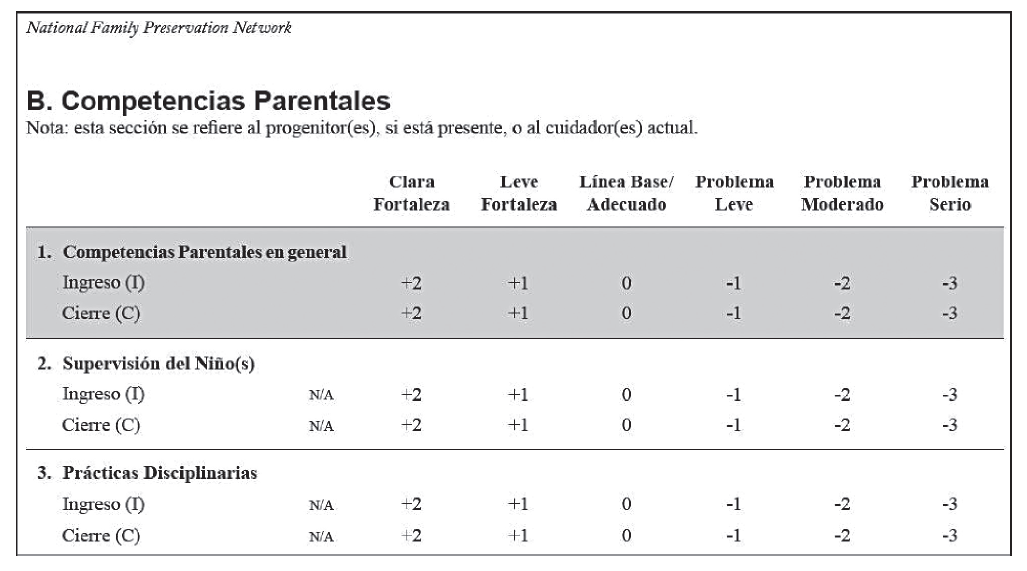
\includegraphics[scale=0.6]{imagenes/NCFAS.png}
	\end{center}
	\caption{Ejemplo Competencias Parentales.}
\end{figure}

\newpage

En la Figura \ref{Figura2} se presenta un ejemplo de las Propiedades Psicométricas de la NCFAS. Donde el profesional encargado de realizar la evaluación necesita revisar cada ítem de cada dimensión para luego evaluar estos ítem según indique las Propiedades Psicométricas de la NCFAS. 
La Figura \ref{Figura2} muestra como ejemplo la dimensión Entorno, ítem "Seguridad de la comunidad". 

\begin{figure}[htb]
	\label{Figura2}
	\begin{center}
		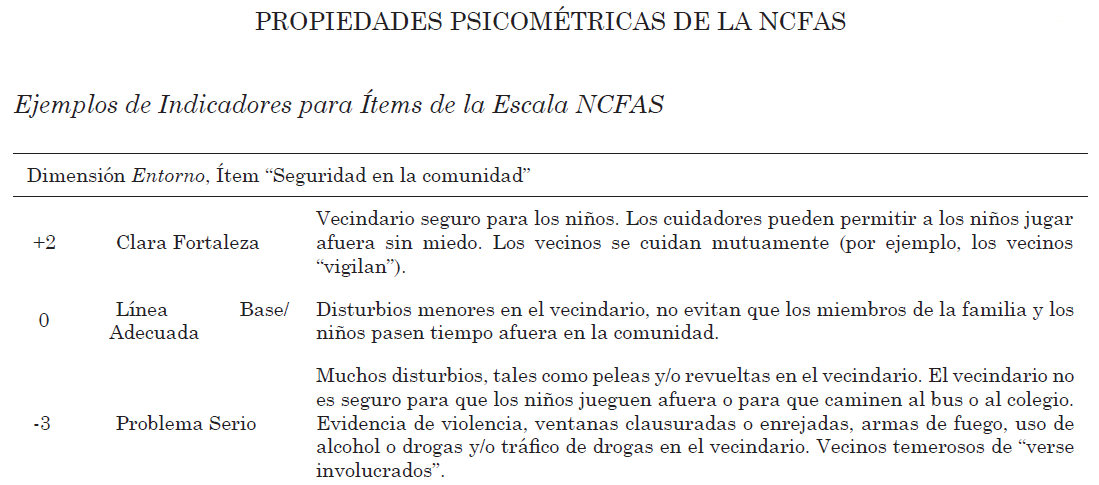
\includegraphics[scale=0.6]{imagenes/propncfas.png}
	\end{center}
	\caption{Ejemplo Propiedades Psicométricas de la NCFAS.}
\end{figure}

\clearpage 


\subsection{Minería de datos}

\subsubsection{Knowliedge Discovery from Data (KDD)}

En palabras simples, minería de datos se refiere a extraer conocimiento desde grandes cantidades de datos. Es por ello que muchas veces se utiliza la palabra minería de datos como un sinónimo de "descubrimiento de conocimiento de los datos". Sin embargo KDD por sus siglas en inglés (Kwnoledge Discovery from Data) es un concepto mucho mas amplio. KDD es un proceso que consta de una serie de pasos y entre uno de ellos se encuentra los pasos esenciales que es la minería de datos.\\
El proceso de descubrimiento de datos consiste en una serie de etapas iterativas, esto significa que es posible volver a ajustar cada etapa anterior si es necesario. En la Figura \ref{Figura3} se ejemplifica las etapas del proceso KDD \cite{han2006data}.

\begin{figure}[htb]
	\label{Figura3}
	\begin{center}
		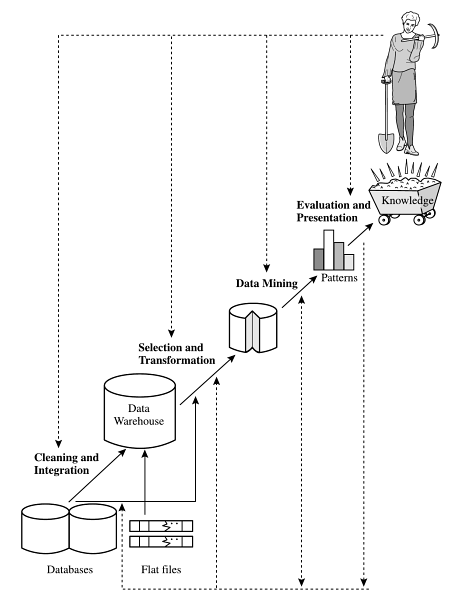
\includegraphics[scale=0.6]{imagenes/kdd2.png}
	\end{center}
	\caption{Ejemplo del proceso KDD.}
\end{figure}

\begin{itemize}
	\item Data cleaning: (Limpieza de datos) Se remueve el ruido y los datos inconsistentes.
	\item Data integration: (Integración) Donde múltiples fuentes de datos pueden ser combinadas.
	\item Data selection: (Selección de datos)  Donde los datos relevantes a la tarea de análisis se recuperan de la base da datos.
	\item Data transformation: (Transformación de los datos) Donde los datos son transformados o consolidados en formas apropiadas preparándolos para la minería de datos.
	\item Data mining: (Minería de datos) En esta etapa se aplican métodos inteligentes con el fin de encontrar patrones de datos. 
	\item Pattern evaluation: (Evaluación de patrones) En esta etapa se evalúan los patrones realmente importantes para cumplir con los objetivos. 
	\item knowlidge presentation: (Presentación del conocimiento) En esta etapa se utilizan las técnicas de representación del conocimiento para presentar al usuario el "conocimiento extraído". 
\end{itemize}

\subsubsection{Minería de datos y sus técnicas}

La Minería de Datos busca encontrar y describir patrones estructurales en los datos y así, servir de herramienta para ayudar a explicarlos, encontrar información interesante  y además, poder hacer predicciones acerca de ellos.

Las técnicas de minería de datos se pueden dividir en : 
\begin{itemize}
	\item \textbf{Aprendizaje supervisado.}
	\item \textbf{Aprendizaje no supervisado}
\end{itemize}
En las técnicas basadas en aprendizaje supervisado se utiliza un conjunto de datos como datos de entrenamiento que están etiquetados y previamente clasificados.\\

En las técnicas basadas en aprendizaje no supervisado los datos a analizar no están clasificados ni etiquetados, por
lo que los algoritmos deben agrupar los datos automáticamente.\\
Dentro de las técnicas de aprendizaje supervisado podemos encontrar:

\begin{itemize}
	\item Clasificación: Es el proceso de encontrar un modelo que describe y distingue clases de datos. El modelo se deriva a partir de un conjunto de datos de entrenamiento, y es usado para predecir el nombre o etiqueta de la clase para objetos que no están clasificados.
	Uno de los algoritmos de clasificación utilizados es el algoritmo TD3, el cual pertenece a la familia TDIDT (Top-Dow Induction of Decision Trees) y su objetivo es construir un árbol de decisión que explique cada instancia de la forma más compacta posible, estableciendo una secuencia dentro del árbol de decisión.\\
	
	\item Reglas de asociación: Son patrones que ocurren frecuentemente en los datos. Estos patrones corresponden a conjuntos de elementos frecuentes, por lo cual, los datos a menudo aparecen juntos dentro de un conjunto de transacciones. Por ejemplo un computador y un software, a menudo cuando la gente compra un computador, existe una gran posibilidad que además compre un software. Pero la gran mayoría de las veces estas asociaciones no son fácilmente detectables. Es por ello que se utilizan algoritmos como por ejemplo el algoritmo apriori. Este algoritmo se basa en el conocimiento previo o apriori de los conjuntos de datos frecuentes.\\
	
	\item Clustering: Esta técnica consiste en agrupar un conjunto de datos u objetos en diferentes subconjuntos o cluster, de tal forma que los objetos que pertenezcan a cada subconjunto sean muy similares entre ellos. Siendo al mismo tiempo diferentes de los objetos pertenecientes a los otros subconjunto. Cada subconjunto o cluster, puede verse como una clase de objetos. Un algoritmo utilizado para realizar clustering es el algoritmo K-means, el cual particiona los datos en K grupos cada uno representado por su centro, donde se determina la distancia entre cada objeto con todos los centros y se agrupan los objetos en base a la distancia mínima a cada cluster. De esta forma se maximiza  la similitud entre los objetos pertenecientes a un mismo cluster.
\end{itemize}



\subsection{Estadística descriptiva}

La estadística descriptiva es un conjunto de procedimientos que tienen por objeto presentar masas de datos por medio de tablas, gráficos y/o medidas de resumen.

\subsubsection{Estadística descriptiva y sus técnicas}

En estadística descriptiva existen una gran variedad de técnicas con el fin de representar los datos de una mejor manera. Algunas de ellas son las que se muestran a continuación.

\clearpage
\newpage

\begin{itemize}

	\item Tablas de frecuencia: Una forma simple de presentar ordenadamente un grupo de observaciones, es a través de la tabla de distribución de frecuencias. La estructura de estas tablas depende de la cantidad y tipo de variables que se están analizando, siendo las más simples las que se refieren a una variable.\\
	
	\begin{figure}[htb]
		\label{Figura4}
		\begin{center}
			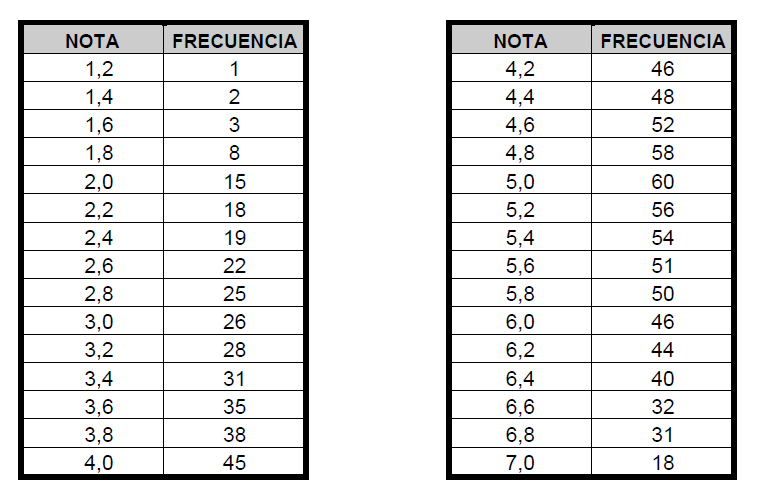
\includegraphics[scale=0.4]{imagenes/tablasdefrecuencia.png}
		\end{center}
		\caption{Ejemplo tablas de frecuencia.}
	\end{figure}
	
\end{itemize}


\begin{itemize}
	\item Histograma: La información además puede representarse gráficamente utilizando histogramas, donde este gráfico representa la frecuencia de un suceso versus el suceso en si.\\
		
	\begin{figure}[htb]
		\label{Figura5}
		\begin{center}
			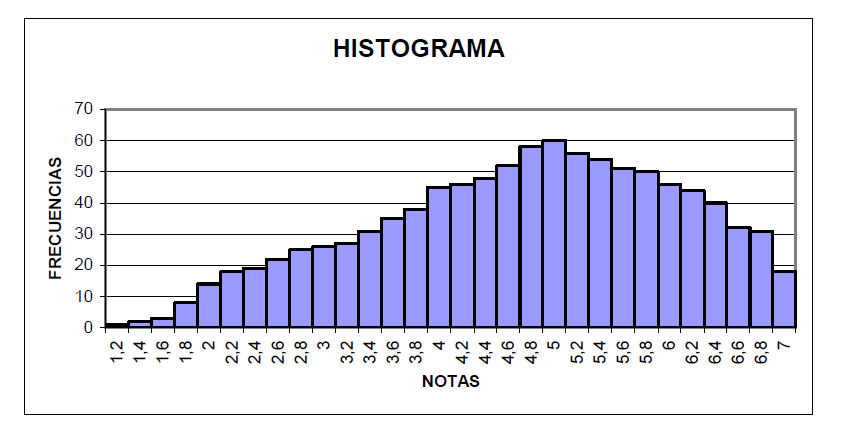
\includegraphics[scale=0.4]{imagenes/histograma.png}
		\end{center}
		\caption{Ejemplo de histograma.}
	\end{figure}
\end{itemize}

\clearpage
\newpage 

\begin{itemize}	
	\item Polígono de frecuencia: Otra forma de representar gráficamente los datos es a través del polígono de frecuencia, el cual es un gráfico de puntos en el cual se muestra la distribución dibujada punto por punto, representando los valores específicos de la variable de estudio.\\

	\begin{figure}[htb]
		\label{Figura6}
		\begin{center}
			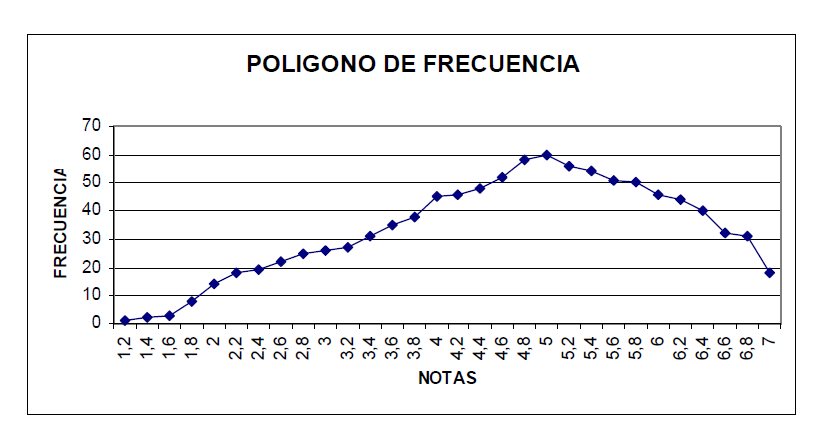
\includegraphics[scale=0.4]{imagenes/poligono.png}
		\end{center}
		\caption{Ejemplo de polígono de frecuencia.}
	\end{figure}
	
\end{itemize}


\section{Técnicas y herramientas existentes}
\label{tec}
\vspace{1mm}
\normalsize

En las investigaciones realizadas actualmente no se han encontrado herramientas similares al sistema propuesto en el Trabajo de Título, esto quiere decir que no se ha encontrado una herramienta publica, ni gratis, ni pagada, que automatice la herramienta NCFAS. Sin embargo es probable que en algunas instituciones manejen algún tipo de sistema similar pero de forma privada. \\ 
A continuación en el punto \ref{tpackage} se presenta un pack de entrenamiento para los profesionales que utilizan NCFAS en papel y en el punto \ref{fbarudy} se muestra una herramienta similar a la escala de evaluación NCFAS. \\ 

Es por ello que no se puede realizar una comparación entre ellas. Sólo se puede realizar una breve comparación entre la escala de evaluación NCFAS y las fichas de Barudy, lo que se detalla en el punto \ref{fbarudy}.  \\
\\
\subsection{NCFAS-G Training Package}
\label{tpackage}
\vspace{2mm}
\normalsize

\begin{figure}[htb]
	\label{Figura7}
	\begin{center}
		
\includegraphics[scale=0.6]{imagenes/nationalfamily.png}
	\end{center}
	\caption{National Family Preservation Network.}
\end{figure}

National Preservation Network (NFPN) es una organización privada encargada de apoyar a otras organizaciones ofreciendo herramientas basadas en la investigación, recursos de capacitación y asistencia técnica. 
Entre ellas ofrece la herramienta NCFAS-G Training Package. Esta herramienta consta de:

\begin{itemize}
	\item Licencia de uso del NCFAS-G + R limitado al número de personas que utilice la herramienta. 
	\item NCFAS-G, Escala y Definiciones
	\item Caso de Estudio con recomendadas Valoraciones y  Formulario
	\item PowerPoint para la Formación del Personal
	\item Respuestas a preguntas frecuentes sobre el uso de la NCFAS-G
\end{itemize}

Cabe mencionar que esta herramienta tiene un costo asociado, dependiendo del número de personas que utilice la herramienta. 

\vspace{2mm}


\subsection{Fichas de Trabajo de Barudy} 
\label{fbarudy}

Las fichas de Barudy, son como su nombre lo dice, fichas para ordenar y estructurar los informes de apreciación familiar, lo que permite focalizar y dirigir la observación. 
Permite además establecer un sustento teórico para enriquecer el análisis y discusión de cada caso. Sin embargo en comparación con NCFAS, las fichas de Barudy resultan ser muy extensas y esto resulta un problema para los evaluadores en los programas de intervención. Este instrumento tampoco ha sido validado científicamente por lo cual no se ha comprobado su efectividad.\\

\clearpage
\newpage

En la Figura \ref{Figura8} se muestra un ejemplo de las fichas de Barudy, en este caso "Valoración de las narrativas de los padres sobre los acontecimientos de sus historias infantiles y familiares que influyen en las competencias parentales" \cite{barudy2010desafios}

\begin{figure}[htb]
	\label{Figura8}
	\begin{center}
		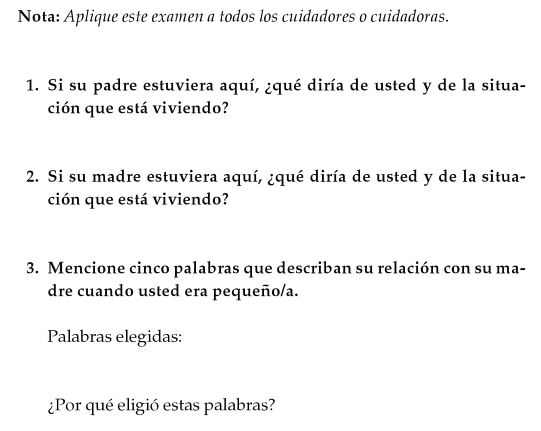
\includegraphics[scale=0.6]{imagenes/fichabarudy.png}
	\end{center}
	\caption{Ejemplo Fichas de trabajo de Barudy.}
\end{figure}
 
 \clearpage
 \newpage
 
\section{Conclusión}

En el Capitulo \ref{mconceptual} se detalla en profundidad el marco conceptual y estado actual de las herramientas digitalizadas de la escala de apreciación NCFAS, que por lo investigado no existen herramientas digitales publicadas al alcance de cualquier institución que apoye a los NNA en riesgo social y sus familias.